%!TEX TS-program = xelatex
\documentclass[a4paper, 12pt]{article}
\usepackage{barinovxesimple}
\geometry{top=25mm}
\geometry{bottom=35mm}
\geometry{left=35mm}
\geometry{right=20mm}
\setlist{labelindent=\parindent,leftmargin=*}
\begin{document}
\thispagestyle{empty}
\begin{center}
    \textit{Федеральное государственное автономное образовательное\\ учреждение высшего образования }

    \vspace{0.5ex}

        \textbf{«Московский физико-технический институт\\ (национальный исследовательский университет)»}
\end{center}

\vspace{10ex}

\begin{center}
    \vspace{13ex}

    \so{\textbf{Лабораторная работа №-.-.-}}

    \vspace{1ex}

    по курсу общей физики

    на тему:

    \textbf{\textit{<<>>}}

    \vspace{30ex}

    \begin{flushright}
        \noindent
        \textit{Работу выполнил:}\\  
        \textit{Баринов Леонид \\(группа Б02-827)}
    \end{flushright}
    \vfill
    Долгопрудный \\2019
\newpage
\setcounter{page}{1}
\fancyhead[R]{\nouppercase{\leftmark}}	
\end{center}

\section{Цель работы}
Исследовать энергетическую зависимость вероятности рассеяния
электронов атомами ксенона. Определить энергии электронов, при
которых наблюдается <<просветление>> ксенона и оценить размер его
внешней электронной оболочки.



\section{Суть исследуемого явления}
Эффект Рамзауэра состоит в аномальном увеличении проницаемости
некоторых газов для весьма медленных электронов. Иными словами, полное
эффективное сечение атома по отношению к проходящему через газ пучку
электронов становится аномально малым при уменьшении их скорости.

\section{Теория явления}
Эффективное сечение реакции --- это величина, характеризующая
вероятность перехода системы двух сталкивающихся частиц в результате
их рассеяния в определенное конечное состояние. Сечение $\sigma$ равно
отношению числа $N$ таких переходов в единицу времени к плотности $nv$
потока рассеиваемых частиц, падающих на мишень, т.е. к числу частиц,
проходящих в единицу времени через единичную площадку, перпендикулярно
к их скорости $v$ ($n$ --- плотность числа падающих частиц)
\begin{equation}
    \sigma = \frac{N}{n v}
    \label{eq:1}
\end{equation}

Рассмотрим схему эксперимента Рамзауэра на \fig{fig:1}

\begin{wrapfigure}{l}{0.4\linewidth}
    \includegraphics[width=\linewidth]{1}
    \caption{Схема установки для измерения сечения рассеяния
    электронов в газах}
    \label{fig:1}
\end{wrapfigure}

Пучок электронов, вылетая из накаленного катода КЛ, проходит
ускоряющую разность потенциалов $V$, приложенную между катодом и
электродом Э, и приобретает тем самым энергию $E=mv^2/2=eV$.
При прохождении через газ часть электронов рассеивается на атомах,
уходит в сторону и собирается коллектором КЛ, а прошедшие без рассеяния
электроны попадают на анод А и создают анодный ток $I$. Ток $I$
пропорционален числу прошедших электронов, и поэтому непосредственно
характеризует проницаемость газа для электронного пучка в зависимости
от его скорости.

Внутри атома потенциальная энергия налетающего электрона $U$ отлиына
от нуля, скорость электрона изменяется, становясь равной $v'$ в
соответствии с законом сохранении энергии
\begin{equation}
    E = \frac{mv^2}{2}= \frac{m v'^2}{2}+U
    \label{eq:2}
\end{equation}
а значит изменяется длина его волны де Бройля. Таким образом, по
отношению к электронной волне атом ведет себя как преломляющая среда с
относительным показателем преломления
\begin{equation}
    n = \frac{\lambda}{\lambda'}=\sqrt{1- \frac{U}{E}}
    \label{eq:3}
\end{equation}
    
Рассмотрим решение задачи о прохождении частицы с энергией $E$ над
потенциальной ямой шириной $l$ и глубиной $U_0$, что будет являться
хорошим приближением для атомов тяжелых инертных газов. 


\begin{figure}[H]
    \floatsetup{heightadjust=object,valign=c}
    \begin{floatrow}

        \ffigbox{
        \caption{Схематическое изображение прямоугольной ямы, над
        которой пролетает частица с энергией $E$}
    }
        {
        \includegraphics[width=0.7\linewidth]{2}
        \label{fig:2}
    }

        \ffigbox{
        \caption{Схема интерференции волн де Бройля при рассеянии на
        атоме}
    }
        {
        \includegraphics[width=0.7\linewidth]{3}
        \label{fig:3}
    }
    \end{floatrow}
\end{figure}

Уравнение Шредингера в данном случае имеет вид
\begin{equation}
    \psi'' + k^2 \psi =0, \hspace{1em} \text{где}\ k^2 = 
    \begin{cases}
        k_1^2 = \dfrac{2mE}{\hbar^2} & - \text{в областях I и III}
        \\[1em]
        k_2^2 = \dfrac{2m (E+U_0)}{\hbar^2} & - \text{в области II}
    \end{cases}
    \label{eq:4}
\end{equation}

Коэффициент прохождения равен отношению квадратов амплитуд прошедшей и
падающей волн и определяется выражением
\begin{equation}
    D = \frac{16k_1^2k_2^2}{16k_1^2k_2^2 + 4 (k_1^2-k_2^2)^2 \sin^2
    (k_2 l)}
    \label{eq:5}
\end{equation}
или
\begin{equation}
    D ^{-1} = 1 + \frac{ (k_1^2 - k_2^2)^2 }{4k_1^2 k_2^2}\sin^2 (k_2
    l) = 1 + \frac{U_0^2}{4E (E+U_0)}\sin^2 (k_2 l)
    \label{eq:6}
\end{equation}

Коэффициент прохождения имеет ряд чередующихся максимумов и минимумов.
Коэффициент максимален при условии

\begin{equation}
    k_2 l = \sqrt{ \frac{2m (E+U_0)}{\hbar^2} }l = n \pi, \hspace{1em} n =
    1, 2, 3\ldots
    \label{eq:7}
\end{equation}

На \fig{fig:3} показано, как волна де Бройля отражается от границ
атомного потенциала, т.е. от поверхности атома, и происходит
интерференция прошедшей через атомы волны $1$ и волны $2$, отраженной
от передней и задней границы атома.

Прошедшая волна $1$ усилится волной $2$, если геометрическая разность
хода между ними $\Delta = 2l = \lambda'$, что соответствует условию
первого интерференционного максимума, т.е. при условии
\begin{equation}
    2l = \frac{h}{\sqrt{2m (E_1 + U_0)}}
    \label{eq:8}
\end{equation}
Здесь $E_1$ --- энергия электрона, соответствующая этому условию,
которое естественно, совпадает с условием \eqref{eq:7}, следующим из
решения уравнения Шредингера.

С другой стороны, прошедшая волна ослабится, если $\Delta = 2l =
(3/2)\lambda'$ (условие первого интерференционного минимума), т.е. при
условии 
\begin{equation}
    2l = \frac{3}{2} \frac{h}{\sqrt{2m (E_2 + U_0)}}
    \label{eq:9}
\end{equation}

Решая совместно эти два уравнения (8, 9), можно исключить $U_0$ и
найти эффективный размер атома $l$
\begin{equation}
    l = \frac{h \sqrt{5}}{\sqrt{32m (E_2 - E_1)}}
    \label{eq:10}
\end{equation}
Энергии $E_1$ и $E_2$ соответствуют энергиям электронов, прошедших
разность потенциалов $V_1$ и $V_2$, т.е. $E_1 = e V_1$ и $E_2 = e
V_2$.

Из формул \eqref{eq:8} и \eqref{eq:9} можно также по измеренным величинам
$E_1$ и $E_2$ рассчитать эффективную глубину потенциальной ямы атома:
\begin{equation}
    U_0 = \frac{4}{5} E_2 - \frac{9}{5} E_1
    \label{eq:11}
\end{equation}






\section{Оборудование}

\subsection{Экспериментальная установка}

%\vspace{-7em}

\begin{figure}[H]
\begin{minipage}[b]{0.4\linewidth}
%\vspace{-7em}
    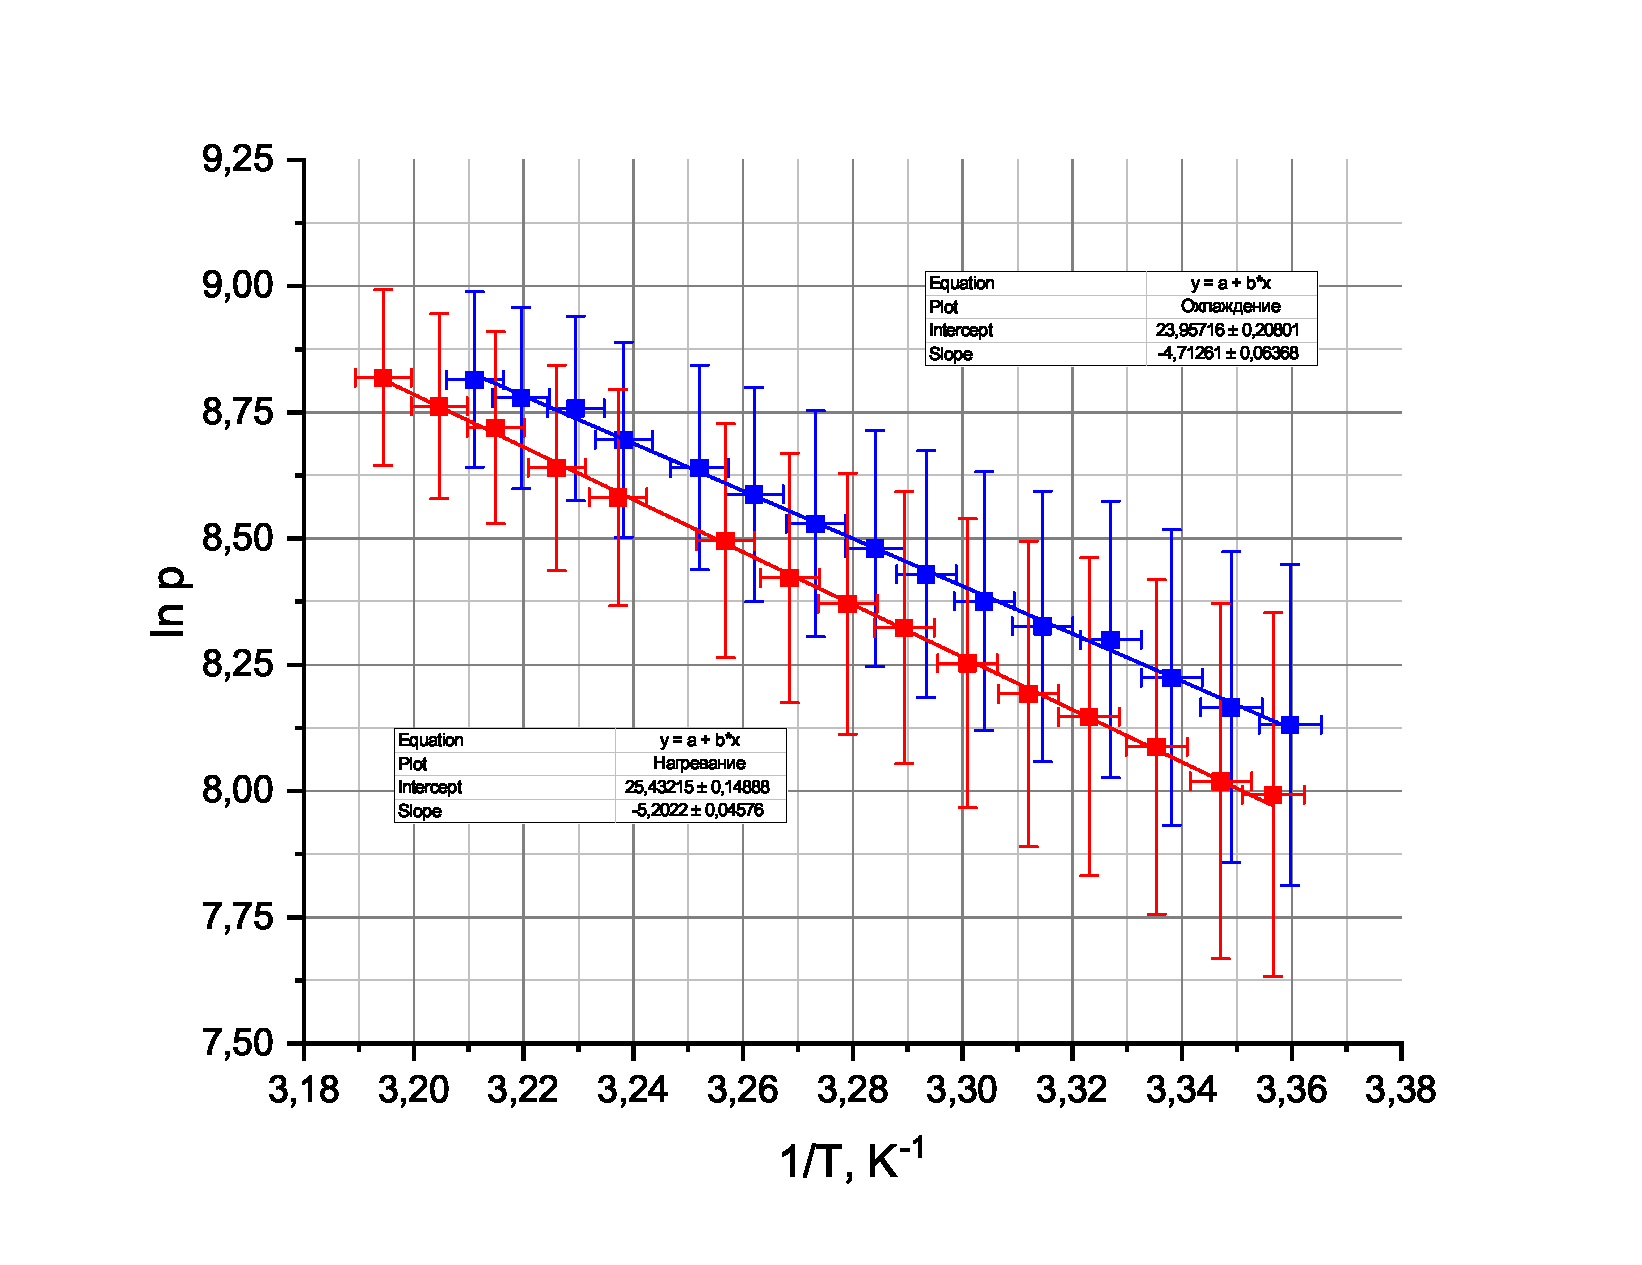
\includegraphics[width=\linewidth]{4}
    \caption{Схематическое изображение тиратрона (слева) и его
    конструкция (справа): 1, 2, 3 --- сетки; 4 --- внешний
металлический цилиндр; 5 --- катод; 6 --- анод; 7 --- накаливаемая
спираль}
\label{fig:4}
\end{minipage}
\end{figure}



В работе используется тиратрон ТГ3-01/1.3Б, заполненный инертным
газом. Схематическое изображение тиратрона и его конструкция приведены
на \fig{fig:4}

Электроны, эмитируемые катодом тиратрона, ускоряются напряжением $V$,
приложенным между катодом и ближайшей к нему сеткой. Затем электроны
рассеиваются на атомах инертного газа. Все сетки 1, 2, 3 соединены
между собой и имеют одинаковый потенциал, примерно равный потенциалу
анода 6. Поэтому между первой сеткой 1 и анодом практически нет поля.
Рассеянные электроны отклоняются в сторону и уходят на сетку, а
оставшаяся часть электронов достигает анода и создаёт анодный ток
$I_a$. Таким образом, поток электронов $N(x)$ на расстоянии $x$ от
ускоряющей сетки уменьшается с ростом $x$ от начального значения $N_0$
у катода (в точке $x=0$) до некоторого значения $N_a$ у анода (в точке
$x = L$).

\begin{wrapfigure}{r}{0.35\linewidth}
    \includegraphics[width=\linewidth]{5}
    \caption{Вероятность рассеяния электрона атомом инертного газа и
    ВАХ тиратрона при квантовом рассмотрении}
    \label{fig:5}
\end{wrapfigure}


Рассмотрим реальную вольт-амперную характеристику тиратрона. Выделим в
газе на расстоянии $x$ тонкий слой с площадью поперечного сечения $S$
в толщиной $dx$. Этот слой содержит $\nu = n_a S dx$ атомов газа
($n_a$ --- концентрация атомов газа в лампе). Суммарная рассеивающая
поверхность этих атомов $\Delta = \nu \Delta_a$, где $\Delta_a$ ---
площадь поперечного сечения атома. Обозначим через $dN$ убыль потока
электронов в результате прохождения слоя $dx$; тогда $dN/N(x)$ есть
доля электронов, которые рассеялись, или вероятность рассеяния в слое.
Для рассеяния электрона в слое необходимо выполнение двух независимых
событий --- электрон должен <<наткнуться>> в слое на атом, и, кроме
того,  он должен на этом атоме рассеяться. Вероятность $dN/N(x)$
рассеяния электрона в слое равна произведению двух вероятностей ---
вероятности для электрона в слое $dx$ встретить атом газа и
вероятности рассеяния на атоме $w(V)$:
\begin{equation}
    - \frac{dN}{N(x)} = -\frac{d N}{N(x)} = \frac{\Delta}{S}w(V) = n_a
    \Delta_a w (V)dx
    \label{eq:12}
\end{equation}

\begin{wrapfigure}[10]{l}{0.4\linewidth}
\vspace{-1em}
    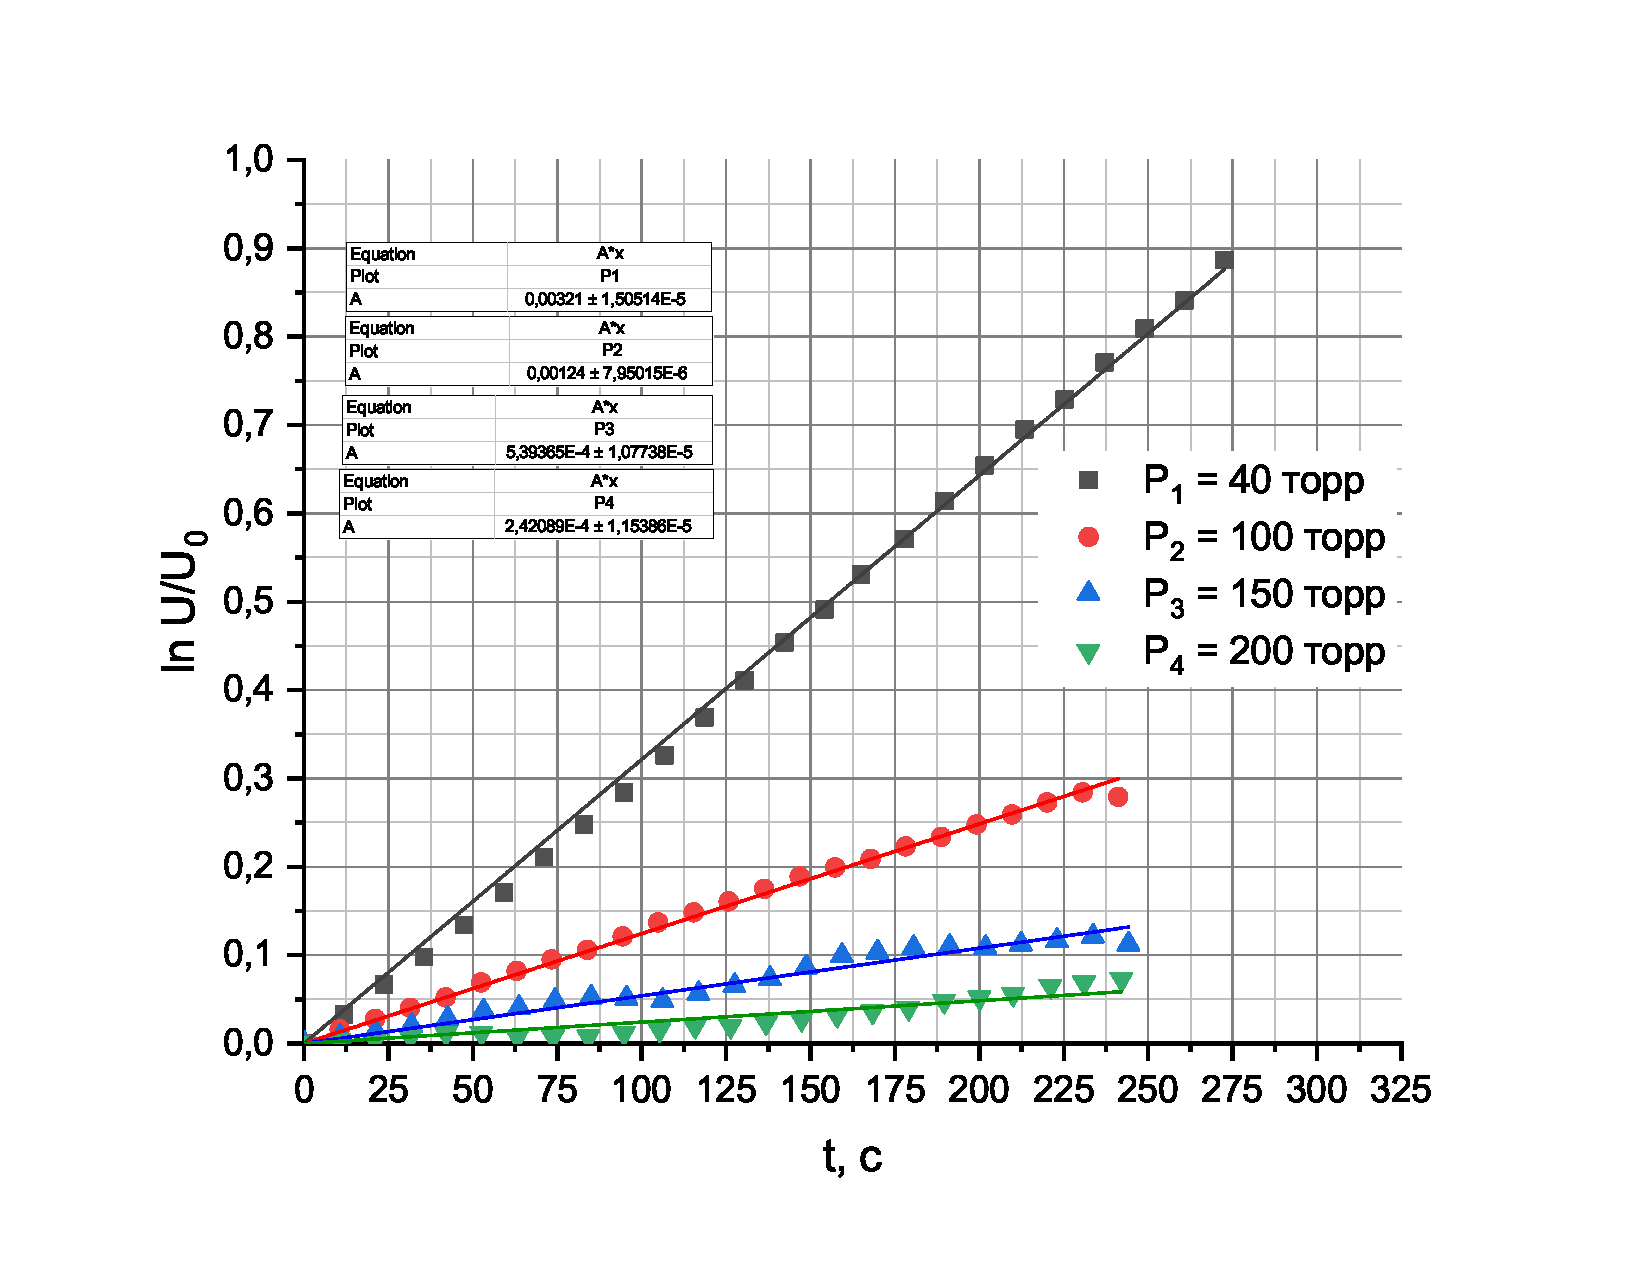
\includegraphics[width=\linewidth]{6}
    \caption{Схема включения тиратрона}
    \label{fig:6}
\end{wrapfigure}

Интегрируя это соотношение от $0$ до $L$ и заменяя поток на ток
$I=Ne$, получаем уравнение ВАХ:
\begin{equation}
    I_a = I_0 e ^{-C w (V)}, \hspace{1em} C = L n_a \Delta_a,
    \label{eq:13}
\end{equation}
где $I_0 = e N_0$ --- ток катода, $I_a = e N_a$ --- анодный ток.

Согласно формуле \eqref{eq:11}, по измеренной ВАХ тиратрона можно
определить зависимость вероятности рассеяния электрона от его энергии
из соотношения
\begin{equation}
    w (V) = -\frac{1}{C} \ln \frac{I_a (V)}{I_0}
    \label{eq:14}
\end{equation}


Принципиальная схема установки для изучения эффекта Рамзауэра
приведена на \fig{fig:6}. На лампу Л подается синусоидальное
напряжение частоты 50 Гц от источника питания ИП, С ---
стабилизированный блок накала катода; исследуемый сигнал подается на
электронный осциллограф (ЭО); цифрами обозначены номера ножек лампы.


\begin{figure}[H]
    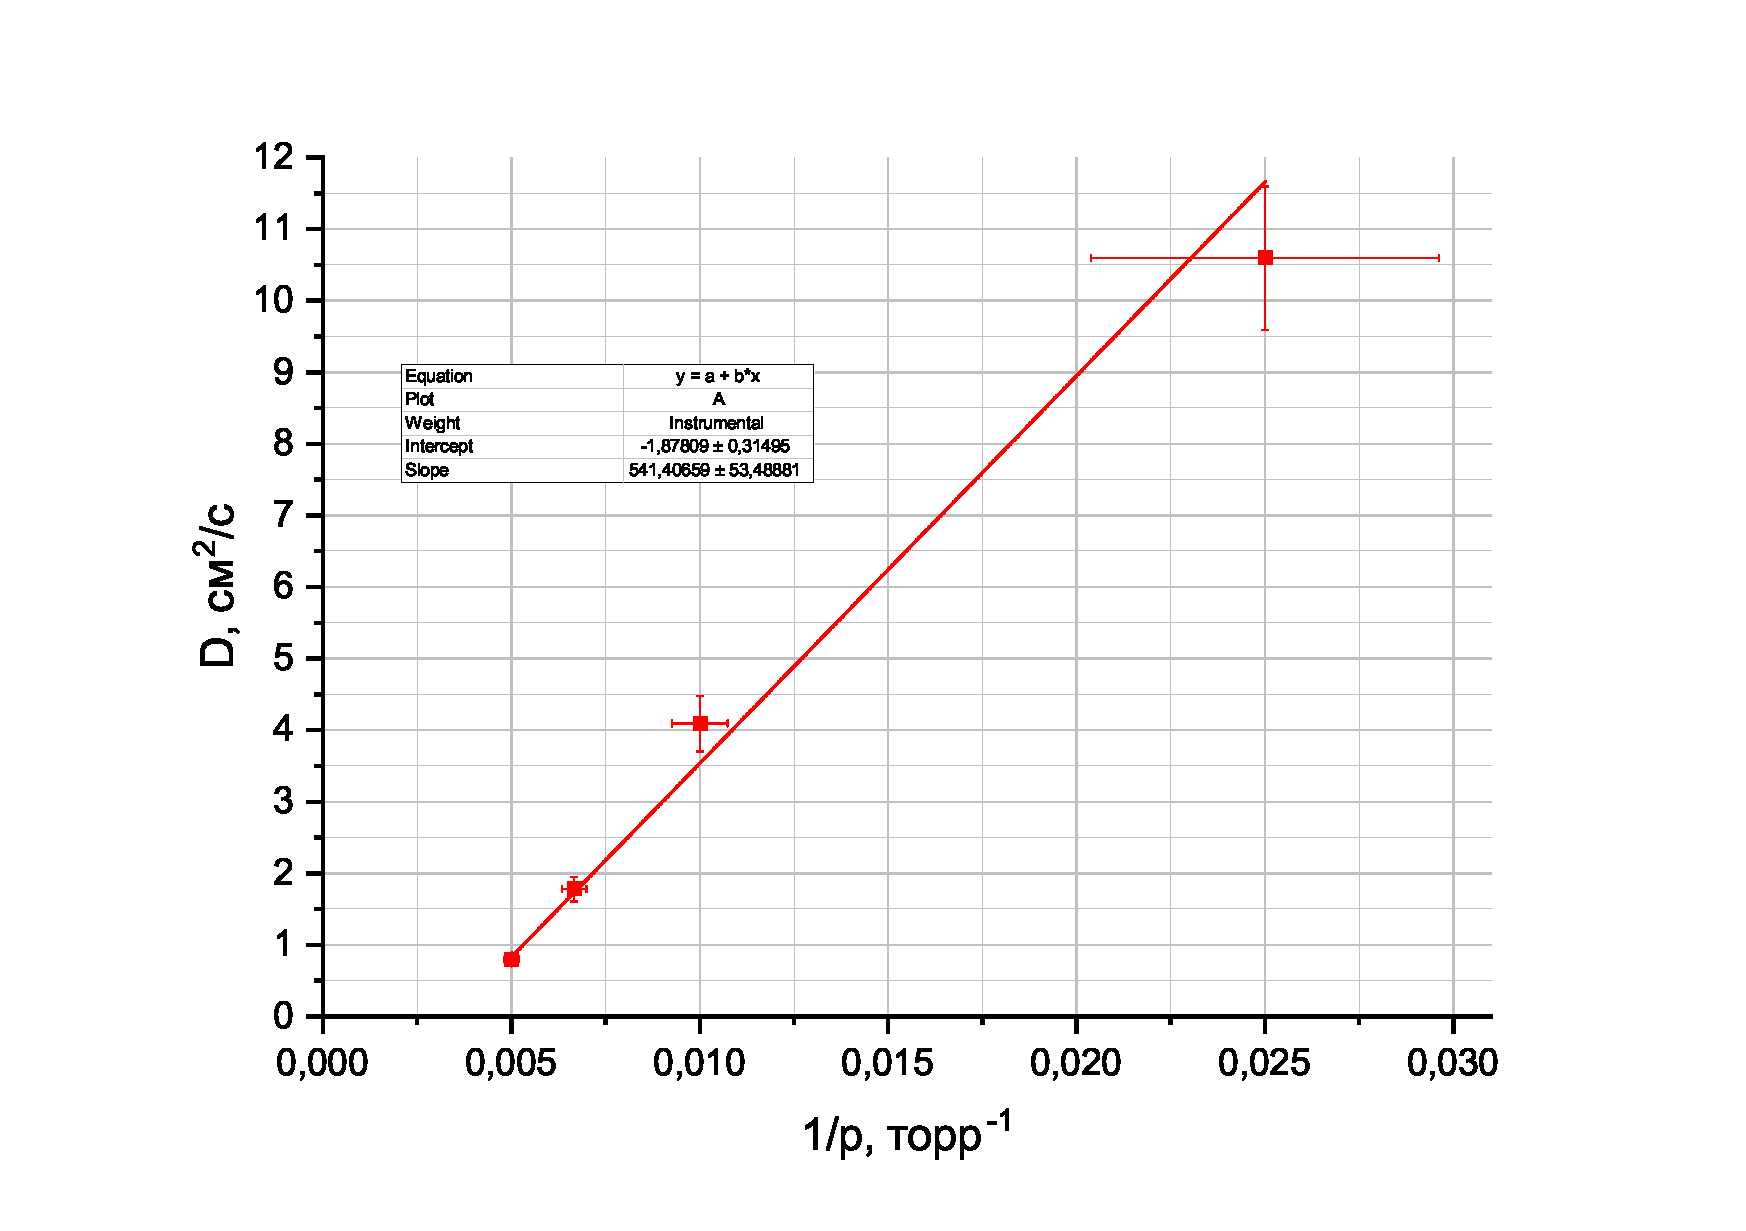
\includegraphics[width=0.8\linewidth]{7} 
    \caption{Блок-схема экспериментальной установки}
    \label{fig:7}
\end{figure}

Схема экспериментальной установки, изображенная на \fig{fig:6} в нашей
работе конструктивно осуществлена следующим образом. Лампа-тиратрон
ТГЗ-01/1.3Б, заполненная инертным газом, расположена непосредственно
на корпусе блока источников питания (БИП). Напряжение к электродам
лампы подается от источников питания, находящихся в корпусе прибора.
Регулировка напряжения и выбор режима работы установки производится
при помощи ручек управления, выведенных на лицевую панель БИП
\ffig{fig:7}.


\section{Результаты эксперимента}
Получим ВАХ тиратрона в динамическом режиме при максимальном
ускоряющем напряжении и различном напряжении накала $V_\text{нак}$:


\begin{figure}[H]
    \floatsetup{heightadjust=object,valign=c}
    \begin{floatrow}

        \ffigbox{
        \caption{Вольт-амперная характеристика тиратрона $V_\text{нак}
        = 2,995\: \text{В}$}
    }
        {
        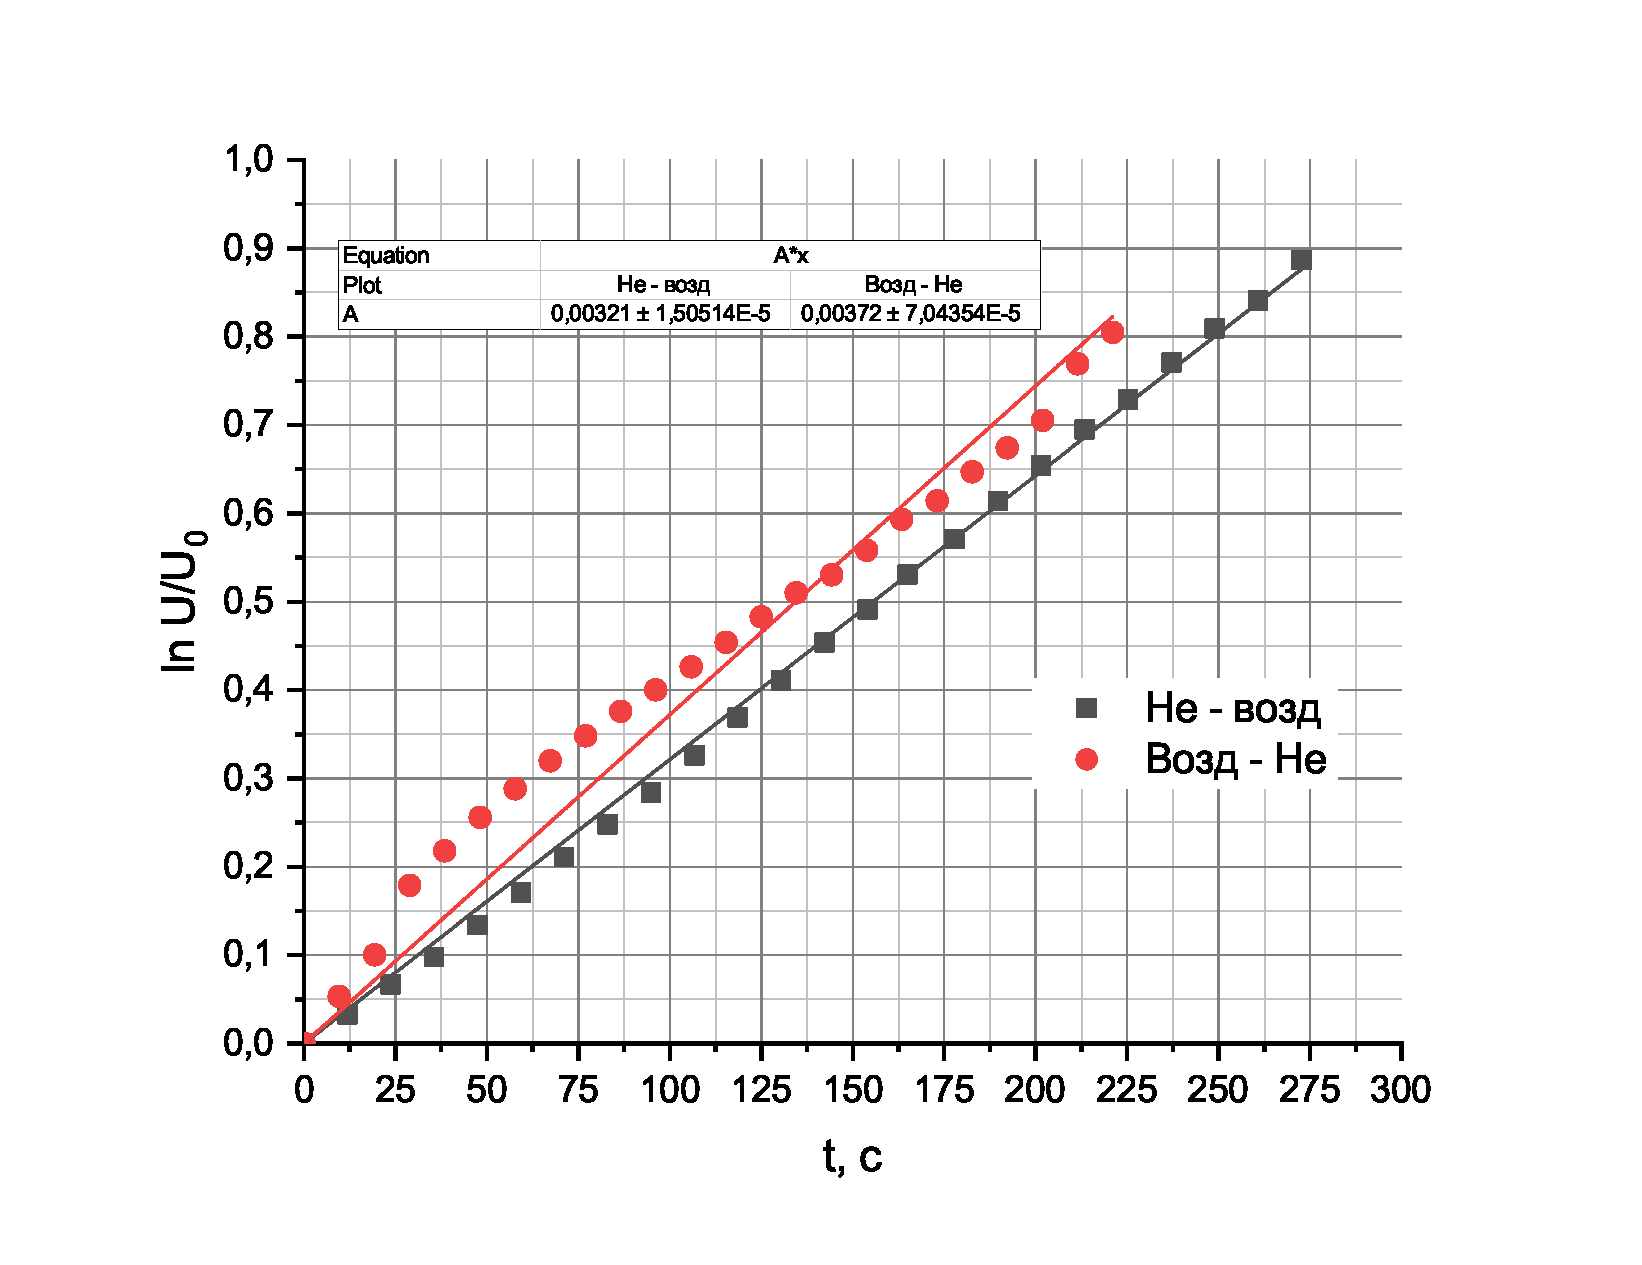
\includegraphics[width=0.9\linewidth]{8}
        \label{fig:8}
    }

        \ffigbox{
        \caption{Вольт-амперная характеристика тиратрона $V_\text{нак}
        = 2,503\: \text{В}$}
    }
        {
        \includegraphics[width=0.9\linewidth]{9}
        \label{fig:9}
    }
    \end{floatrow}
\end{figure}

Измерим напряжение $\Delta V$, соответствующие первому максимуму и
минимуму на осциллограмме.
\[
    \Delta V = (3,7 \pm 0,6)\: \text{В}
\]

Снимем вольт-амперную характеристику $I_a = f(U_c)$ в статическом
режиме.


\renewcommand{\arraystretch}{1.4}
\begin{table}[H]
\centering
\begin{tabular}{|c|c|c|c|c|c|cc}
\hline
\multicolumn{4}{|c|}{$V_\text{нак} = 2,503\: \text{В}$}
& \multicolumn{4}{c|}{$V_\text{нак} = 3,018\: \text{В}$}                                                   \\ \hline
$I_a,\: \text{мкА}$    & $U_c,\: \text{В}$      & $I_a,\: \text{мкА}$         & $U_c,\: \text{В}$         & $I_a,\: \text{мкА}$     & $U_c,\: \text{В}$      & \multicolumn{1}{c|}{$I_a,\: \text{мкА}$}     & \multicolumn{1}{c|}{$U_c,\: \text{В}$}     \\ \hline
0,002 & 0,113  & 1,698      & 2,004     & 1,346 & 3,209  & \multicolumn{1}{c|}{1,620} & \multicolumn{1}{c|}{1,977} \\ \hline
0,302 & 0,635  & 1,594      & 2,168     & 1,231 & 4,639  & \multicolumn{1}{c|}{1,568} & \multicolumn{1}{c|}{1,976} \\ \hline
1,474 & 1,250  & 1,631      & 2,117     & 1,322 & 5,893  & \multicolumn{1}{c|}{1,394} & \multicolumn{1}{c|}{1,940} \\ \hline
1,677 & 1,510  & 1,656      & 2,080     & 1,504 & 6,862  & \multicolumn{1}{c|}{1,207} & \multicolumn{1}{c|}{1,793} \\ \hline
1,316 & 2,426  & 1,711      & 1,984     & 1,960 & 8,299  & \multicolumn{1}{c|}{1,127} & \multicolumn{1}{c|}{1,685} \\ \hline
0,798 & 3,426  & 1,809      & 1,657     & 2,874 & 9,839  & \multicolumn{1}{c|}{0,731} & \multicolumn{1}{c|}{0,828} \\ \hline
0,586 & 4,487  & 1,792      & 1,546     & 4,116 & 11,334 & \multicolumn{1}{c|}{0,598} & \multicolumn{1}{c|}{0,515} \\ \hline
0,535 & 5,013  & 1,657      & 1,348     & 1,273 & 4,061  & \multicolumn{1}{c|}{0,500} & \multicolumn{1}{c|}{0,332} \\ \hline
0,509 & 5,477  & 1,326      & 1,136     & 3,807 & 1,292  & \multicolumn{1}{c|}{0,422} & \multicolumn{1}{c|}{0,220} \\ \hline
0,500 & 6,172  & 0,847      & 0,921     & 4,481 & 1,249  & \multicolumn{1}{c|}{0,335} & \multicolumn{1}{c|}{0,129} \\ \hline
0,504 & 6,727  & \multicolumn{2}{c|}{$V_\text{нак} = 3,018\: \text{В}$} & 5,264 & 1,260  & \multicolumn{1}{c|}{0,270} & \multicolumn{1}{c|}{0,083} \\ \hline
0,526 & 7,444  & 0,020      & 0,122     & 4,787 & 1,245  & \multicolumn{1}{c|}{0,207} & \multicolumn{1}{c|}{0,050} \\ \hline
0,582 & 8,396  & 1,382      & 0,972     & 2,176 & 1,770  & \multicolumn{1}{c|}{0,002} & \multicolumn{1}{c|}{0,006} \\ \hline
0,781 & 9,826  & 1,851      & 1,916     & 1,855 & 1,918  & \multicolumn{1}{c|}{0,077} & \multicolumn{1}{c|}{0,014} \\ \hline
1,330 & 11,935 & 1,584      & 2,463     & 1,690 & 1,966  &                            &                            \\ \cline{1-6}
\end{tabular}\caption{Вольт-амперная характеристика тиратрона при
различном напряжении накала $V_\text{нак}$}
\end{table}





\section{Анализ результатов}

В формуле \eqref{eq:10} рассчитаем эффективный размер атома $l$:
\[
    l = (3,6 \pm 0,3)\: \mathring{A}
\]

Оценим глубину потенциальной ямы по формуле \eqref{eq:11}:
\[
    U_0 = (1,6 \pm 0,2)\: \text{эВ}
\]

Напряжению пробоя $V \approx 13\: \text{В}$, определенному из
\fig{fig:8} и \fig{fig:9}, лучше всего соответствует газ ксенон с
ионизационным потенциалом $12,1\: \text{В}$ (по сравнению с криптоном
и ксеноном).

Построим ВАХ тиратрона для статического режима \ffig{fig:10}. По
графику определим эффективный размер атома $l$:
\[
    l' = (3,6 \pm 0,2)\: \mathring{A}
\]

Также оценим глубину потенциальной ямы по формуле \eqref{eq:11}:
\[
    U_0' = (1,3 \pm 0,3)\: \text{эВ}
\]


\begin{figure}[H]
    \includegraphics[width=0.9\linewidth]{10} 
    \caption{Вольт-амперная характеристика тиратрона для двух
    напряжений накала}
    \label{fig:10}
\end{figure}

Оценим, используя формулу \eqref{eq:7} при каких напряжениях должны
появляться максимумы в коэффициенте прохождения электронов для $n = 2,
3$.
\begin{equation*}
    \begin{gathered}
        E_2 \approx 10\: \text{эВ}\\
        E_3 \approx 25\: \text{эВ}
    \end{gathered}
\end{equation*}

На основе формулы \eqref{eq:14} найдем зависимость вероятности
рассеяния электронов (с точностью до константы) от энергии и построим
соответствующий график:


\begin{figure}[H]
    \includegraphics[width=0.9\linewidth]{11} 
    \caption{Зависимость вероятности $w$ рассеяния электронов от
    напряжения $U_c$}
    \label{fig:11}
\end{figure}




\section{Выводы}
В работе было проведено исследование эффекта Рамзауэра. Построены
вольт-амперные характеристики тиратрона в динамическом
\textsl{(рис.~\ref{fig:8}, рис.~\ref{fig:9})} и статическом
\ffig{fig:10} режимах
работы. На ВАХ отчетливо видно наличие локального минимума и
локального максимума, что соответствует рассмотрению взаимодействия
электронов с атомами с квантовой точки зрения \ffig{fig:5}. График
вероятности $w$ рассеяния электронов от напряжения \ffig{fig:11} также
соответствует квантовому описанию эффекта \ffig{fig:5}. 

По максимуму и минимуму на ВАХ рассчитаны эффективные размеры атома
газа $l$ и проведена оценка глубины потенциальной ямы $U_0$ (значения
в динамическом и статическом режимах близки друг к другу).
\begin{equation*}
    \begin{gathered}
        l = (3,6 \pm 0,3) \mathring{A}\\
        U_0 = (1,5 \pm 0,3)\: \text{эВ}
    \end{gathered}
\end{equation*}

Значения отличаются от табличных:
\begin{equation*}
    \begin{gathered}
        l^\text{т} = 2,8\: \mathring{A}\\
        U_0^\text{т} = 2,5\: \text{эВ}
    \end{gathered}
\end{equation*}

Расхождения связаны с упрощенным рассмотрением эффекта и техническими
неточностями установки. Формула
\eqref{eq:5} была получена на прямоугольной яме (а не на сферической),
минимумы коэффициента прохождения 
определены из условия $\sin (k_2 l) = 1$, что не совсем
точно, так как величина $4(k_1^2-k_2^2)^2$ зависит от энергии
электрона $E$. Кроме этого стоит отметить, что
при различных напряжениях накала $V_\text{нак}$ значения локального
минимума $V_2$ значительно отличаются \ffig{fig:10}, что является
некорректным и привело к большим погрешностям.

По осциллограммам на \fig{fig:8} и на \fig{fig:9} можно определить
напряжение пробоя $\approx 13\: \text{В}$, что достаточно близко к
ионизационному потенциалу ксенона $12,1\: \text{В}$.

По формуле \eqref{eq:7} была получена оценка энергий электронов, при
которых теоретически могли бы наблюдаться максимумы коэффициента
прохождения 2-го и 3-го порядка. 
\begin{equation*}
    \begin{gathered}
        E_2 \approx 10\: \text{эВ}\\
        E_3 \approx 25\: \text{эВ}
    \end{gathered}
\end{equation*}

Из-за пробоя данные значения на ВАХ не наблюдаются.















\end{document}
